\chapter{計算実験}\label{computational_result}
\section{計算環境}
実験に用いるプログラムはPythonを用いて実装し, 計算機はMacBookAir(CPU: Apple M1 chip, メモリ: 8GB)を用いて行った. 

\section{第一段階の求解結果}
整数計画ソルバー (Gurobi Optimizer ver. 9.5)を用いて計算した結果, 全ての問題例で最適解が得られた. 
出力の例を図\ref{first-no-rei}に示す. 
長方形内の番号はグループの番号を表す. 
灰色の長方形は, ランプを表す. \\

\begin{figure}[b]
    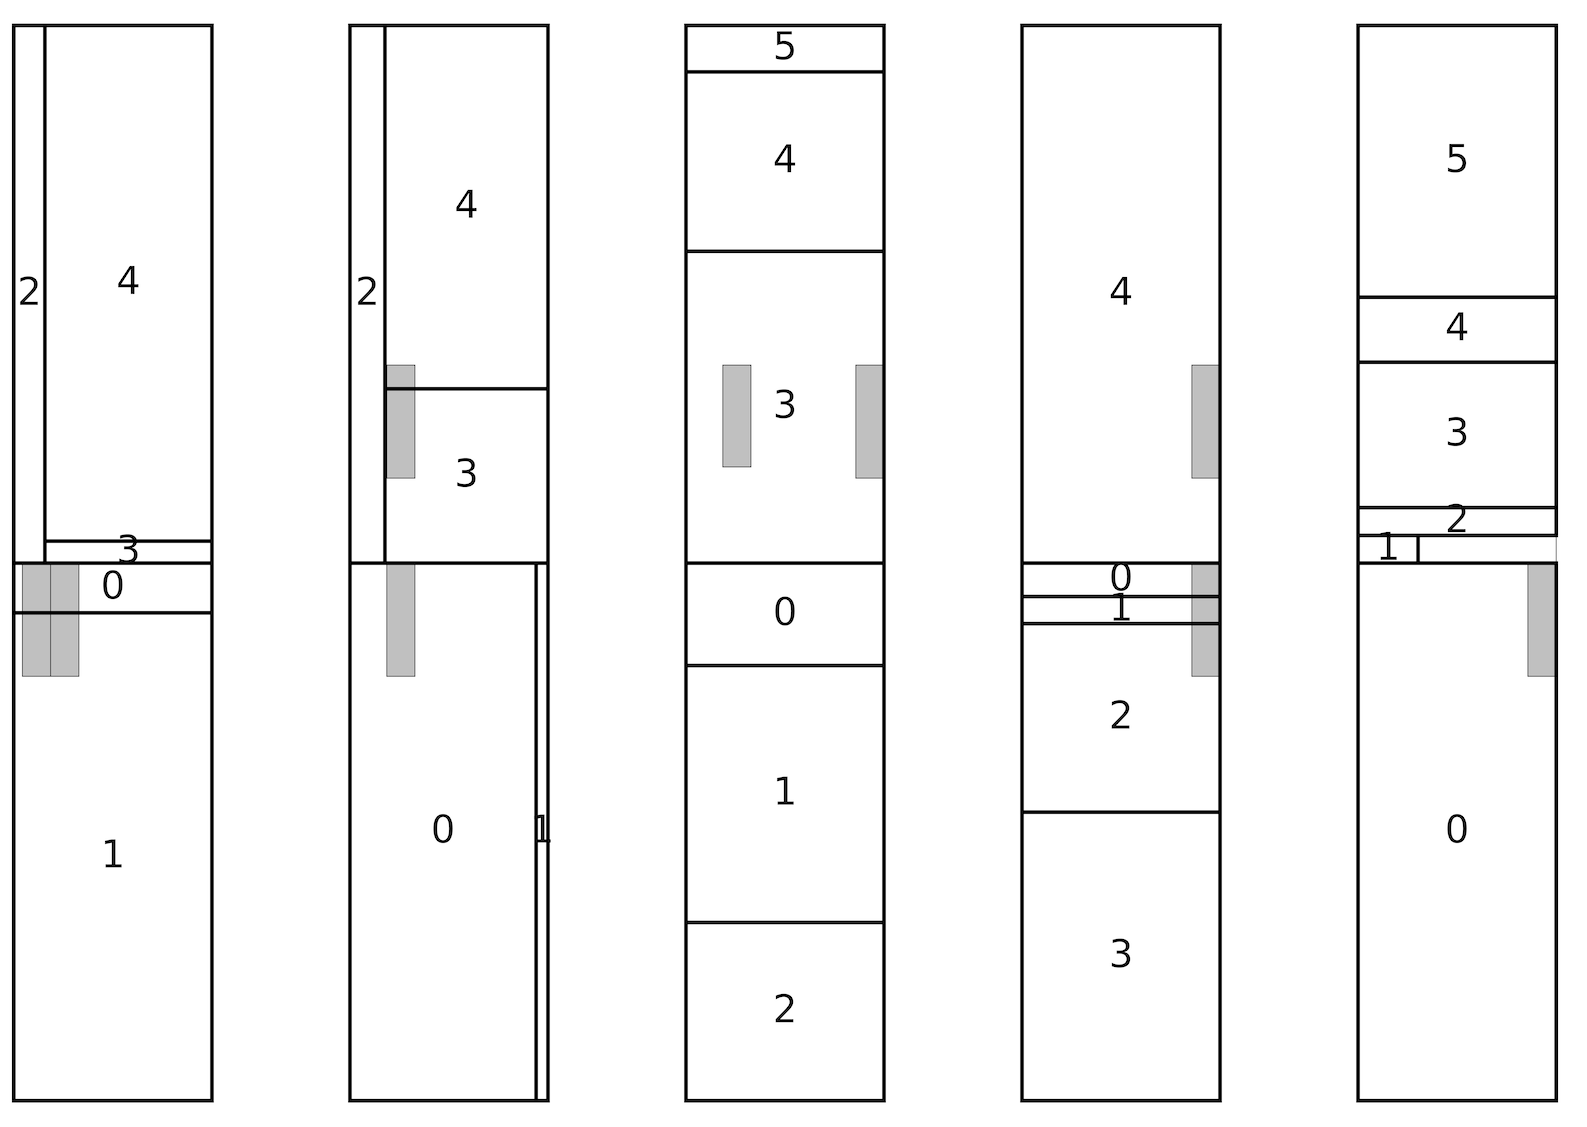
\includegraphics[scale=0.3, bb = 0 0 1 1]{5-first-no-rei.png}
    \caption{第一段階の出力の例}
    \label{first-no-rei}
\end{figure}
\clearpage

\section{第二段階の求解結果}
出力される配置図を図\ref{second-no-rei}に示す. 
各長方形が車を表し, 色は積み地の種類を表す. \\

\begin{figure}[b]
    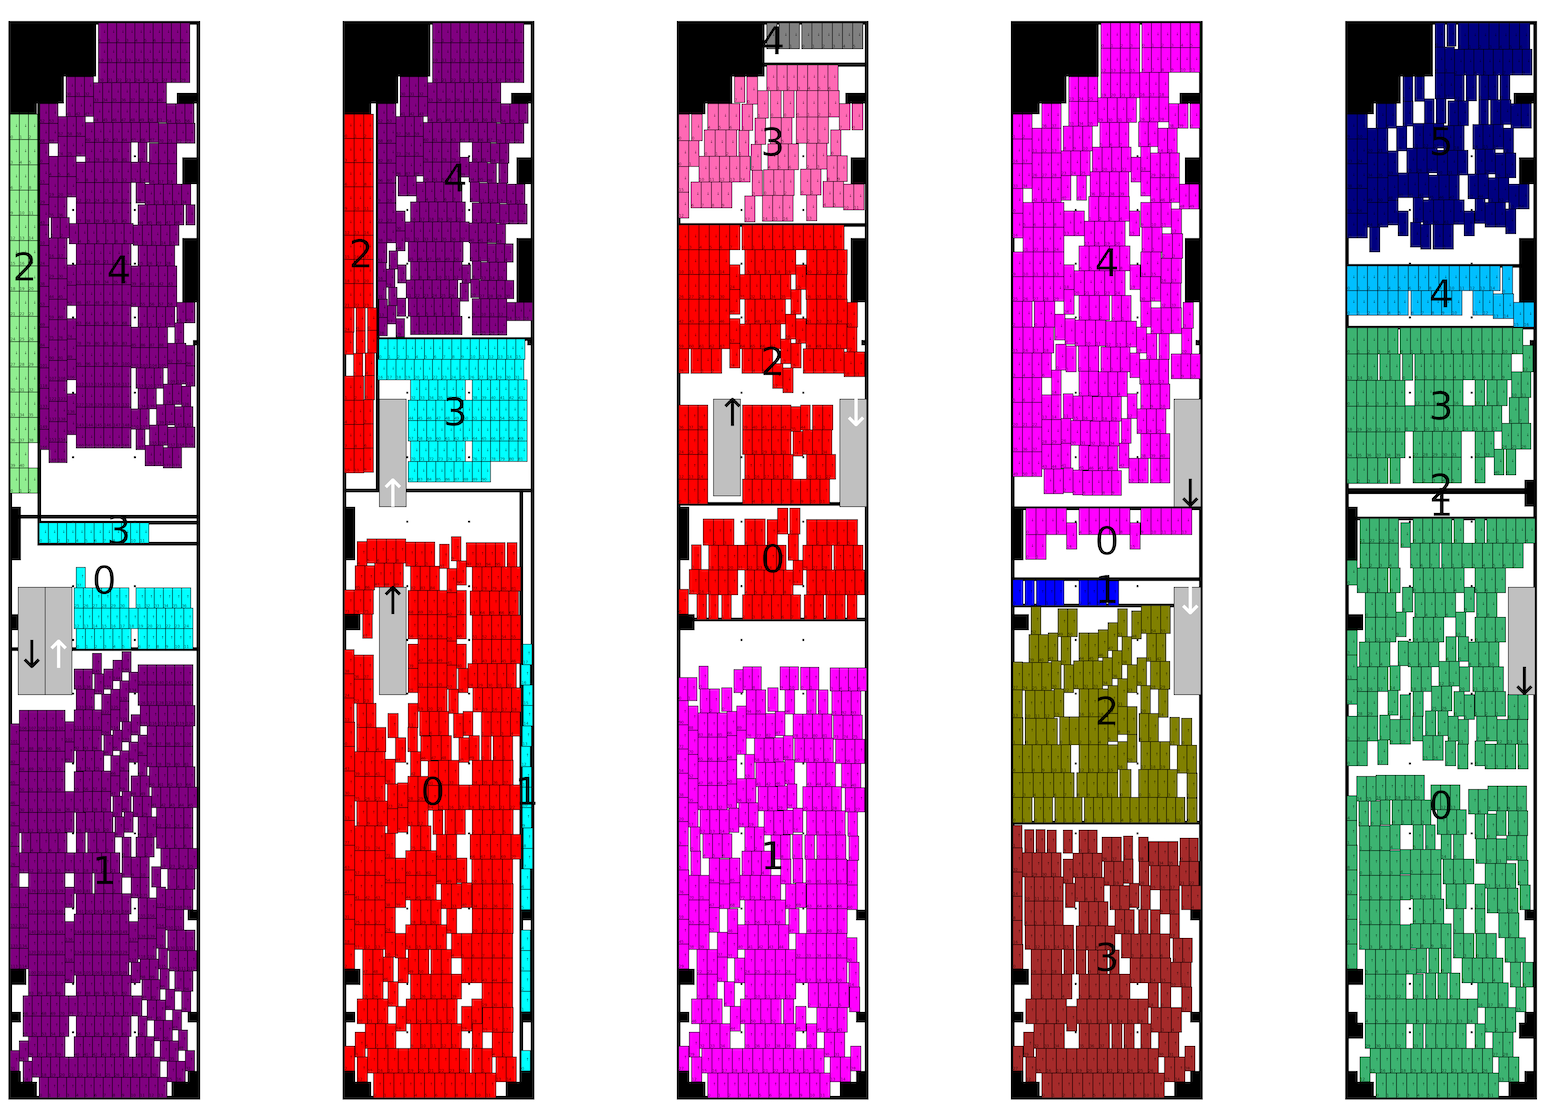
\includegraphics[scale=0.3, bb = 0 0 1 1]{5-second-no-rei.png}
    \caption{第一段階の出力の例}
    \label{second-no-rei}
\end{figure}

